\section {Background: Ecology and Ecosystems}

The credit for coining the word "ökologie" is generally given to Ernst Haeckel who in 1866 suggested that this term should refer to the study of nature's economy. Ecological thinking does not have a history of only 160 years, nevertheless. Haeckel likely drew from Linnaeus’ 18th century conception of the “economy of nature” \citep{worster_1977}. Furthermore, if we consider a modern definition of ecology as "... the study of the structure and function of nature, it being understood that mankind is a part of nature" we can trace the lineage of ecological thought back to classical Greece \citep[][p. 3]{odum_1953}. 

Indeed, in the history of thought concerning humans and their relationships with nature, we find the persistence of three general questions. What is nature's influence on man? What is man's influence on nature? Is there a grand purpose in these relationships\citep{glacken_1967}? Stated in a more ecological sense, these questions can be rephrased. What is the influence of the non-living environment on living organisms? What is the influence of living organisms on the non-living environment? Did God create the earth?

For most of history we have struggled with the first question. Only with the thinking of Darwin did we begin to take it seriously that non-human organisms could be influenced by their surrounding environment. With the recent attention to the Anthropocene we have engaged more deeply with the second question. While it is easy to observe relatively small-scale human influences on the environment, we now understand that both human and non-human life alter the environment at planetary scales. The importance of the third question from Glacken is diminishing in academic circles and is generally left to the theologians, yet holistic (dare we say non-scientific) approaches may be just as important to understanding nature as the concepts of stocks and flows of material resources borrowed from economic thought. 

But we digress, the concept of the ecosystem is the object of inquiry. The term ecosystem was introduced in 1935 by Arthur Tansley, an ecologist frustrated with the use of organismic metaphors to describe biotic communities and their environs (see figure 1). This frustration also extended to applying the organismic metaphor to “human communities as habitually so constituted.” His goal in coining the term was to clarify the notion that the "ecosystem" is an \textit{abstraction} of climate, earth, and life that does not exist outside of human thought \citep{tansley_1935}. An ecosystem is understood as a community of living organisms--the \textit{biocoenosis}: plants, animals, fungi, and so on--and the set of relationships between organisms and with their surrounding non-living environment--the \textit{biotope} \citep{tansley_1935,odum_1953}. Living communities, natural environs, and relationships--ecosystems. 

To confuse matters the term ecology has recently come to refer to simply the relationships found in an ecosystem \citep{oed_2008}. One of the difficulties with the information ecosystem metaphor is this confusion of ecologies with ecosystems. For purposes of clarity in this essay the term(s) ecology(ies) will be used in the original sense to refer to the study(ies) of ecosystems--unless explicitly noted otherwise--not the communities and sets of relations found within an ecosystem. 

\subsection{Early ecosystems and evolution}

Evolution, competition, and cooperation have been applied to ecosystem thinking since its inception, although not without difficulties and ideological differences. As originally conceived by Darwin, evolution was largely competitive; individuals from certain species were in constant struggle to claim and maintain their places in nature's economy. His theory of "descent with modification" was developed in the context of Malthusian thinking on human populations in which food resources increase in a linear fashion and population increases in a exponential manner; quickly competitive survival becomes "red in tooth and claw" not only between species, but within the same species \citep{stoddart_1966,tennyson_1849}.\footnote{the Tennyson poem originally refers to human relationships!} 

Darwin's idea of competitive evolution was quickly adopted to explain phenomena in human societies and "the survival of the fittest" was applied to both the relations between humans and between humans and the environment. The first with dire consequences as shown with Hitler's adoption of the notion of \textit{lebensraum}--in which political nation-states are said to "evolve" and claim spaces in the global economy--to justify his crusade to exterminate the Jews. The second in environmental management rhetoric in which it is our destiny as humans to control and dominate nature \citep{stoddart_1966,worster_1977}. 

Notions of competition do not preclude ideas of symbiosis or mutualism in the evolution of species, nevertheless. At the turn of the 20th century there were thinkers such as Hermann Reinheimer, Petr Kropotkin, and Eugenius Warming who attempted to highlight cooperation and symbiosis as essential strategies for survival in the competitive world \citep{worster_1977}. For example, Petr Kropotkin's work emphasized the cooperative aspects of evolution in both biological and human communities \citep{kropotkin_1902}. While his work was heavily flawed, his thesis leads to current explanations of mutualism in which species co-evolve and rely on one-another to survive. 

Not coincidental, these thinkers all used the economy of nature metaphor to include human economic organization in the conversation. No matter that Kropotkin was an anarchist, these ideas were instilled in the work of the later reductionists (see below) and ecology took on the appearance of a subordinate field of economics and econometrics. The ecosystem is understood as a mirror of human economic production and consumption in which the self-reliant competitor is a but a romanticized idea borrowed from withering frontier ideologies; cooperation is the norm, not competition \citep{worster_1977}.

\subsection{The quantitative revolution: holism and reductionism}

As the nascent field of ecology entered into the post WWII quantitative revolution, ecologists sought to claim an identity as data driven scientists. Arguing in philosophical debates that pitted holism vs. reductionism and organismic vs. mechanistic explanations of nature were central to the work of the ecologist \citep{barbour_1996}. A key proponent of the holistic approach was Frederick Clements who claimed that ecosystems were wholes that were greater than the sums of their parts. He also claimed that entire ecosystems "evolved" along an observable succession of steps to maturity. Thus a particular combination of soil, climate and organisms will always proceed to a defined stable endpoint \citep{clements_1936}. 

Henry Gleason, on the other hand, promoted the view that there is no ecosystem and that all "plant associations" (his term for plant communities or ecosystems) are made of \textit{individuals} competing for resources and space \citep{gleason_1939}.  Gleason also paid particular attention to the problem of scale in ecology and how the scale of analysis determines how an observing scientist will classify an association of plants. Ecologists still profess four main scales in ecology: organism, population, community, and landscape \citep{odum_1953}. Career choices are made based on the scale of study which can determine whether holism or reductionism is the preferred view of natural processes.

Clements' view led to a (non-quantifiable) holistic approach and that of Gleason led to a (quantifiable) reductionist approach \citep{barbour_1996,worster_1977}. With the post-war preference for quantitative work in scientific funding agencies, the reductionist approach gained the most currency; ecology began to be identified as a hard science. By the end of the 1960's the emphasis on quantification led to a "new ecology" in which the principal object of study was the flow of energy and nutrients through the ecosystem \citep{worster_1977,barbour_1996}. 

The nature as machine metaphor had won out over the nature as organism metaphor \citep{hagen_1992}. Yet as prominent ecologist CS Holling recently observes, the analytical [reductionist] approach tends to come up with "exactly the right answer to the wrong question" while the integrative [holistic] approach asks "exactly the right question but [produces a] useless answer" \citep[][p. 3]{holling_1998}. From another perspective John Cantlon explains that "The individualistic community [reductionist] is likely to remain the more useful paradigm for most work understanding ecosystem processes. However ... for landscape interpretation and management purposes, we will undoubtedly continue to the ... taxonomic community [holistic]" \citep[Cantlon 1996, cited in ][p. 241]{barbour_1996}.

This debate is far from over in ecology and it is articulated with similar debates in the academy writ large. This is one area where the "information ecosystem" metaphor is very powerful; there is a constant tension between epistemological approaches of understanding how parts function and understanding how wholes function. At the extreme poles of this debate some claim that "everything is connected to everything" \citep{commoner_1971} while others claim that a particular cause leads to a specific effect. As Sir Karl Popper suggested through another metaphor, science struggles to classify things--especially the human body and mind--as either clocks or clouds in the quest to understand rationality, free will, and the importance of information and how it affects the material world through human action. 

\subsection{Information Diversity and Biodiversity}

Parallel to this reductionist-integrative debate in ecology novel theories of information and communication emerged from work at Bell Labs and other growing technology firms. With the advent of digital computers during the war, and the subsequent interest in \textit{securely} managing larger and larger sets of information, people began to speak of and study the "information environment." 

One of the key problems that was addressed in this work was the diversity of information in a data stream; this was particularly important on noisy channels for the transmission of data on metal wires (think telephone and telegraph lines). A major advance was made by the work of Claude Shannon at Bell Labs who proposed a mathematical theory of information diversity \citep{shannon_1948}. His text is still considered canonical in computer and information science. Ecologists also picked it up and started to use the same methods for calculating diversity of food webs or \textit{trophic diversity} \citep{macarthur_1955} and then for the diversity of organisms themselves in an ecosystem \citep{margalef_1957}. 

Margalef was "fully conscious ... of the risk of displeasing both mathematicians and biologists" with the application of diversity models from information theory to ecosystem biodiversity. He was also aware that this mathematical model for biodiversity was far from perfect \citep{margalef_1957}. Shannon's diversity index is still taught to students of ecology as part of a standard set of methodological tools, nevertheless. This is an important early and direct direct link between information science and ecology.

\subsection{Dynamic equilibrium and Chaos Theory}

In early ecological thinking the ecosystem evolved through several stages to a reach a final stable state. This concept of an "evolved" ecosystem is now debunked and instead "dynamic equilibriums" are used to describe states which ecosystems tend to gravitate toward. 

Crafword Holling's twin concepts of systemic resistance to change and the resilience of a system after a major disturbance are often used to explain dynamic equilibriums in ecosystems. When observing populations of organisms that either compete for knowable quantities of resources (plant communities) or are in predator-prey relationships (animal communities) the demographics tend to hover around a stable point unless there is a disturbance (fire, weather event, human intervention, and so on) \citep{holling_1973}. 

The ecosystem modeler Robert May questioned the idea of stable points in population dynamics and introduced the possibility of using chaotic models to explain observed population phenomena in ecosystems.\footnote{Ecosystem modeling was then a very new field that used computers to model species populations in a study ecosystem} He demonstrated that with sufficient disturbance the model may gravitate to more than one stable point similar to strange attractors in chaos theory, or the system may bifurcate and enter periods of instability \citep{may_1974}. 

This approach drew heavily from cybernetic systems theory, the notion of the \textit{self-governing} system with a complex of negative and positive feedback loops that led to emergent properties of the system in question. In a strange enigma, the cybernetic-mechanistic approach led to complexity theory and finally back to holistic approaches to describe ecosystems as unknowable wholes \citep{barbour_1996}.

\subsection{Ecology and sustainable resource management}

Sustainability is directly related to stability and systems-based thinking. As examples, the roles of competition, cooperation, synergism and co-dependency can be articulated with sustainability. Each is explored briefly.

First, a limiting resource, such as Nitrogen (food) or light (energy), may govern the behaviour of the system; especially if competition for the resource exists. The "carrying capacity" of an ecosystem for some species can be calculated based on a limiting resource. This simple calculation is very seductive yet it hides several dangers. Due to vagaries of the weather, natural and non-natural disturbances, and so on, it is nearly impossible to calculate a carrying capacity. Furthermore, when the calculation is applied to human populations "lifeboat ethics" come into play. Instead of seeking political solutions to manage resources, the only solution is to limit human reproduction. Hard questions immediately arise as to who lives and who dies.

Second, ecosystem structure and function is thought to be sustained by "keystone species" which, if removed from the living community, may cause the ecosystem to spiral toward a different dynamic equilibrium. By definition the keystone species has one or more cooperative or synergistic relations with other organisms in the environment. The removal causes a \textit{trophic cascade}--a catastrophic breakdown of the flows of energy and matter in the ecosystem. Note that humans cannot be considered as a keystone species as they do not always maintain ecosystems, instead they tend to degrade them. 

Third, predator-prey populations have a co-dependent relationship where cause and effect are bi-directional. Once again humans cannot be considered predator nor prey for management reasons. It could imply either the encouragement of breeding or the culling of human populations, that latter of which is unthinkable for most. 

These three ideas represent some of the well-worn tools in the management of ecosystems, whether used to calculate the optimum number of ruminants for an area of land, to protect keystone species under law, or to restore once decimated predator populations to control a prey population. 

Striking is that even after the idea of the evolved stable ecosystem was laid to rest, many ecologists still seek stability in natural ecosystems as a form of sustainable management. While there is a popular belief that biodiversity begets stability through increased resistance and resilience to systemic disturbance, the evidence is split. In artificially closed study systems--through choice of scale or boundaries--diversity may beget stability, yet in open systems concepts of thresholds, chaos, and tipping points may be more useful \citep[for opposing arguments see][]{tilman_1994,goodman_1975}. Furthermore, in 1978 Joseph Connel proposed the still relevant thesis that the highest rates of biodiversity are maintained with intermediate rates of disturbance. \citep{connel_1978}. 

Yet most interventions to conserve and maintain biodiversity involve setting land aside and minimizing disturbance. Only recently have we realized that conservation as preservation. A novel alternative proposal is found in the Panarchy literature in which humans and human organizations are explicitly considered as \textit{parts} of an ecosystem. Holling's 1973 ideas of Resistance and resilience are then applied to these broad socio-natural environments to make not only recommendations for ecological interventions that include moderate disturbance regimes (controlled burns for example), but also to make recommendations for political interventions \citep{holling_2002}.

\subsection{The ecologist as a manager, activist, and agent of change}

In a short time "ecology" and "ecosystem" have become important parts of the English language and are considered household terms in addition to the more academic uses outlined above (see figure 1). In addition to deepening our understandings of natural processes, ecologists have also given rise to an environmental ethic. The writings of Aldo Leopold \citep{leopold_1949}, Rachel Carson \citep{carson_1962}, Paul Ehrlich \citep{ehrlich_1968} and Barry Commoner \citep{commoner_1971} are often cited as influential in initiating the environmental movement of the 1970s. While all of their works are flawed, these researchers contributed to the idea of the \textit{academic activist} in the realm of protecting and conserving the natural environment. 
 
 \begin{figure}[!ht]
  \centering
    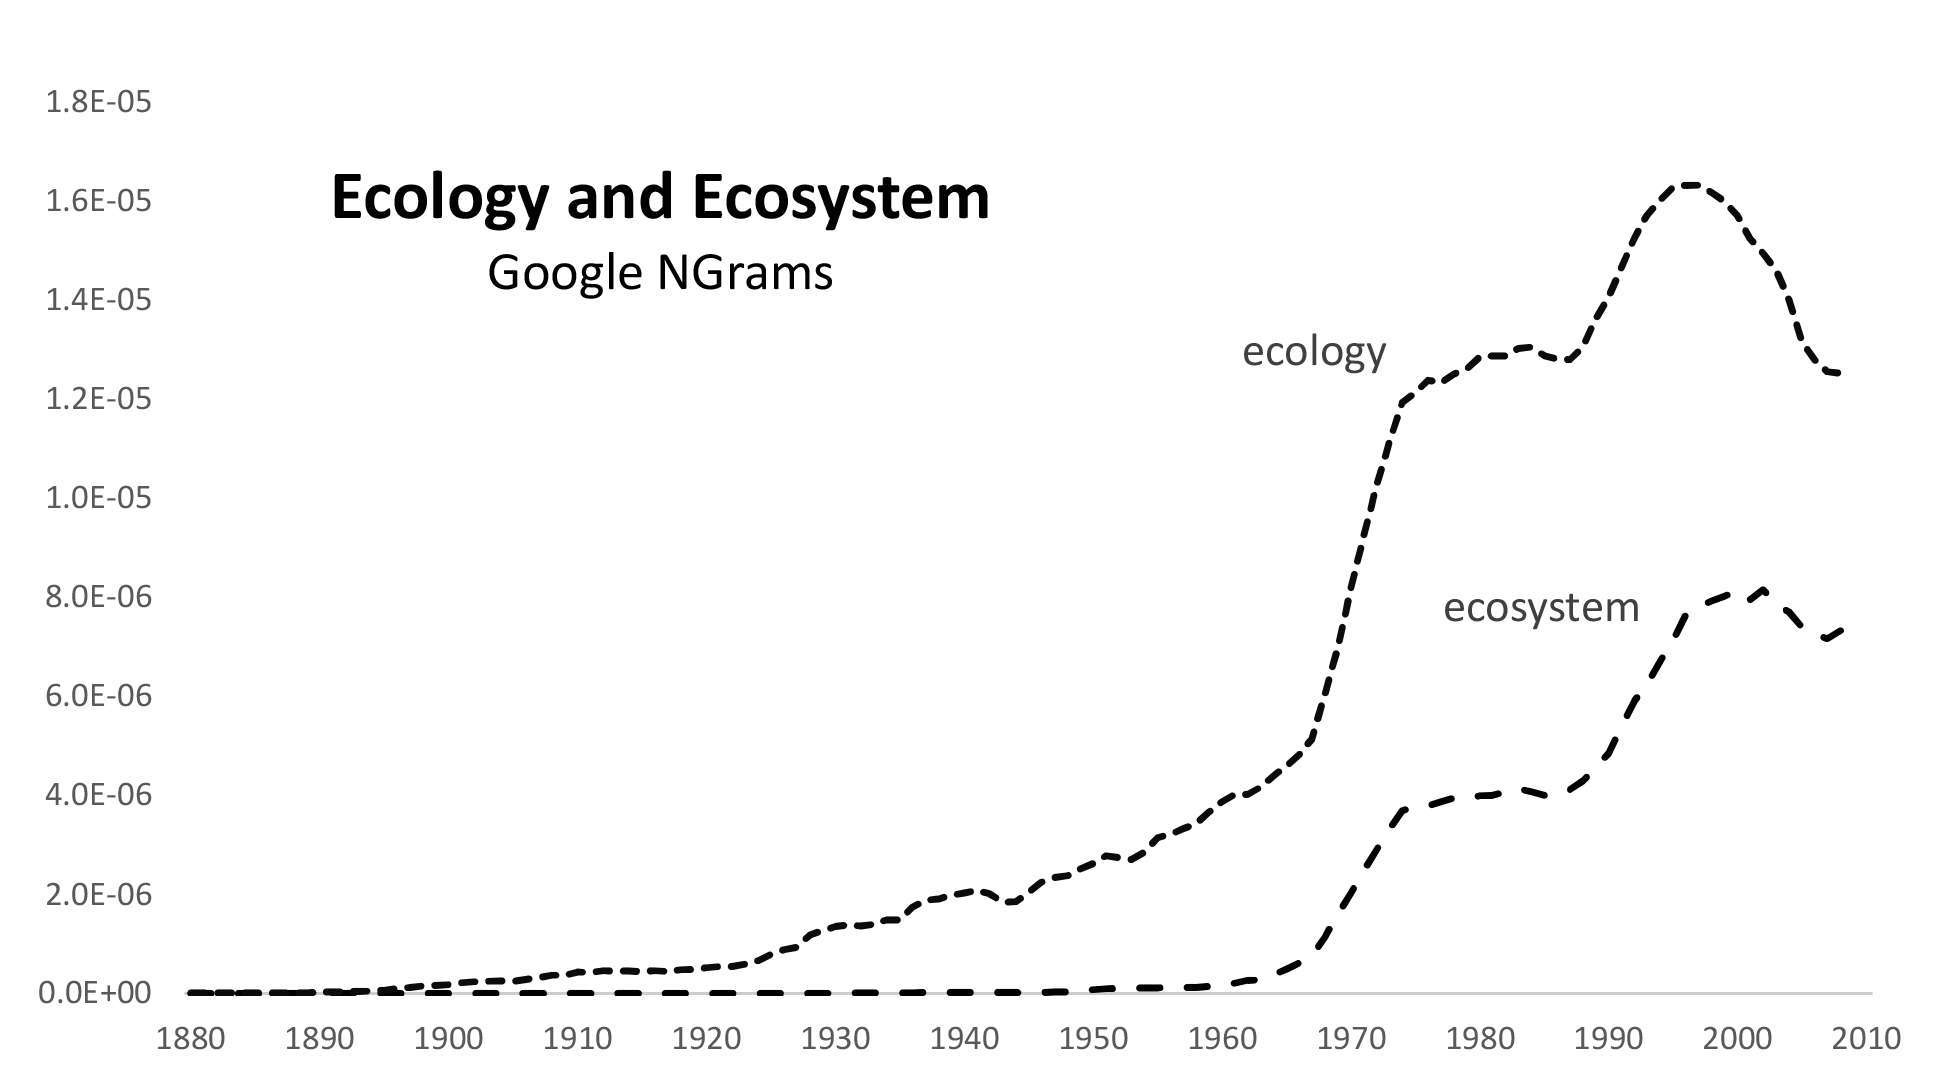
\includegraphics[width=5.5in]{figures/ecologyEcosystem}
  \caption{The emergent use of the words "ecology" and "ecosystem" as a Google Ngram. The rise in the 1970s is attributable to the first Earth Day and the birth of the environmental movement. The second rise in the 1990s can be attributed to broader use of ecological metaphors outside of ecology (see figure 2).}
\end{figure}
 
As writers, they were also fundamental in promoting two key principals in the environmental movement. First, that man is a part of nature and not outside of or above natural law. Leopold stated clearly that "The land ethic . . . simply enlarges the boundaries of the [human] community to include soils, waters, plants, and animals, or collectively the land" \citep[][p. 204]{leopold_1949}. And second, that there may be planetary limits to economic growth. One of the key pieces of literature, the Club of Rome Report, or \textit{The Limits to Growth}, is based on a computer model of population and resources at a planetary scale \citep{meadows_1972}. It represents an early and important intersection of data science, computational models, global ecology, and sustainable resource management.
 
Ecology is now a cornerstone of environmental management. Much of the environmental management literature draws from ecological concepts and "adaptive management" is promoted as a means to improve both social and environmental outcomes of planned interventions \citep{holling_1978,leopold_1963}. Adaptive management iterates planning, action, evaluation and modification as an ongoing process to accommodate shifting environmental and social factors. An equally important emphasis is to bring people back into the sustainable management of ecosystems; conservation on productive landscapes \citep{berkes_2000,holling_2002}. 

In this managerial vein the information ecosystem metaphor resonates powerfully with ecological thinking and adaptive management. Are there "information ecologists" who are key actors in the sustainable management of digital resources? Could these people be considered keystone species in an information ecosystem?